\documentclass{article}
\usepackage[utf8]{inputenc}
\usepackage{polski}
\selecthyphenation{polish}
\usepackage{graphicx}
\usepackage{hyperref}
\usepackage{amsmath}
\usepackage{tikz}

\title{Wielościany}
\author{Damian Lechański i Rafał Motyka}
\date{\today}

\begin{document}

\maketitle

\abstract{
\textbf{Wielościan} - bryła geometryczna, ograniczona przez tak zwaną powierzchnię wielościenną, czyli powierzchnię utworzoną z wielokątów o rozłącznych wnętrzach i każdym boku wspólnym dla dwóch wielokątów.
\newline
\textbf{Wielościan} to figura geometryczna, która:
\begin{itemize}
\item jest ograniczona,
\item jest domknięta,
\item jest wypukła,
\item zawiera co najmniej jeden punkt wewnętrzny,
\item jej brzeg jest sumą skończonej liczby wielokątów.
\end{itemize}
Wielokąt możemy również określić używając pojęcia \textbf{zamkniętej powierzchni wielościanu}, która jest figurą utworzoną z wielokątów leżących w różnych płaszczyznach tak, że każdy z boków jest wspólny dla dwóch wielokątów. Każdy taki wielokąt to \textbf{ściana}, a boki i wierzchołki wielokąta nazywamy \textbf{bokami i wierzchołkami} powierzchni wielościennej. Wówczas \textbf{wielościan to figura geometryczna ograniczona powierzchnią wielościenną}.
}

\tableofcontents

\newpage

\section{Siatka wielościanu}
\textbf{Siatka wielościanu} jest to rozwinięcie powierzchni danego wielościanu na płaszczyźnie, po "rozcięciu" wielościanu wzdłuż odpowiednich krawędzi. Dany wielościan może mieć kilka różnych siatek. Siatki stosujemy, gdy chcemy wykonać model wielościanu.

\section{Elementy wielocianów foremnych}
\begin{table}[h]
\centering
\begin{tabular}{||l|c|c|c||}
\hline\hline
Nazwa & Liczba ścian i ich kształt & Liczba krawędzi & Liczba wierzchołków \\ \hline
czworościan & 4 trójkąty & 6 & 4 \\
sześcian & 6 kwadratów & 12 & 8 \\
ośmiościan & 8 trójkątów & 12 & 6 \\
dwunastościan & 12 pięciokątów & 30 & 20 \\
dwudziestościan & 20 trójkątów & 30 & 12 \\
\hline\hline
\end{tabular}
\caption[Elementy wielościanów foremnych]{\label{tab.elementyWieloscianow}Elementy wybranych wielościanów foremnych}
\end{table}

\section{Przykładowe wielościany}
\subsection{\href{https://pl.wikipedia.org/wiki/Sze\%C5\%9Bcian_(geometria)}{Sześcian}}
Sześcian \ref{fig:szescian} jest bryłą, którą tworzy sześć jednakowych kwadratów, więc ma 12 równych krawędzi. Przekątne ściany są tej samej długości na wszystkich ścianach. Przekątne bryły – złącze wierzchołków, które nie leżą na jednej ścianie – są również tej samej długości.
\newline
Pole powierzchni sześcianu można obliczyć ze wzoru \ref{eqn.szescianPole}, a objętość \ref{eqn.szescianObjetosc}.
\begin{figure}[h]
\centering
\setlength{\unitlength}{1cm}
\begin{picture}(4,4)(0,0)
\put(0,0){\line(0,1){3}}
\put(0,0){\line(1,0){3}}
\put(3,0){\line(0,1){3}}
\put(0,3){\line(1,0){3}}

\put(1,1){\line(0,1){3}}
\put(1,1){\line(1,0){3}}
\put(4,1){\line(0,1){3}}
\put(1,4){\line(1,0){3}}

\put(0,0){\line(1,1){1}}
\put(0,3){\line(1,1){1}}
\put(3,0){\line(1,1){1}}
\put(3,3){\line(1,1){1}}

\put(1.5,0.1){$a$}
\put(2.7,1.5){$a$}
\put(3.6,0.35){$a$}
\end{picture}
\caption{\label{fig:szescian}Sześcian}
\end{figure}

\begin{equation}
\label{eqn.szescianPole}
\mathrm{P}=6a^2
\end{equation}

\begin{equation}
\label{eqn.szescianObjetosc}
\mathrm{V}=a^3
\end{equation} 

\newpage
\subsection{\href{https://pl.wikipedia.org/wiki/Walec_(bry\%C5\%82a)}{Walec}}
Walec \ref{fig:walec} jest bryłą składającą się z dwóch równoległych podstaw i płaszczu. Płaszcz jest prostopadły do podstawy, a podstawa jest utworzona przez koło.
\newline
Pole powierzchni walca można obliczyć ze wzoru \ref{eqn.walecPole}, a objętość \ref{eqn.walecObjetosc}.
\begin{figure}[h]
\centering
\setlength{\unitlength}{1cm}
\begin{picture}(3,5)(0,0)
\qbezier(0,0.5)(0.1,0.9)(1.5,1)
\qbezier(3,0.5)(2.9,0.9)(1.5,1)
\qbezier(0,0.5)(0.1,0.1)(1.5,0)
\qbezier(3,0.5)(2.9,0.1)(1.5,0)

\qbezier(0,4.5)(0.1,4.9)(1.5,5)
\qbezier(3,4.5)(2.9,4.9)(1.5,5)
\qbezier(0,4.5)(0.1,4.1)(1.5,4)
\qbezier(3,4.5)(2.9,4.1)(1.5,4)

\put(0,0.5){\line(0,1){4}}
\put(3,0.5){\line(0,1){4}}
\put(0,0.5){\line(1,0){1.5}}

\put(0.7,0.6){$r$}
\put(2.7,2){$h$}
\end{picture}
\caption{\label{fig:walec}Walec}
\end{figure}

\begin{equation}
\label{eqn.walecPole}
\mathrm{P}=2\pi r(r+h)
\end{equation}

\begin{equation}
\label{eqn.walecObjetosc}
\mathrm{V}=\pi r^2h
\end{equation} 

\newpage
\subsection{\href{https://pl.wikipedia.org/wiki/Kula)}{Kula}}
Kula \ref{fig:kula} jest określona promieniem lub średnicą, jest zbiorem punktów, które są odległe od środka maksymalnie długością równą promieniowi.
\newline
Pole powierzchni kuli można obliczyć ze wzoru \ref{eqn.kulaPole}, a objętość \ref{eqn.kulaObjetosc}.
\begin{figure}[h]
\centering
\setlength{\unitlength}{1cm}
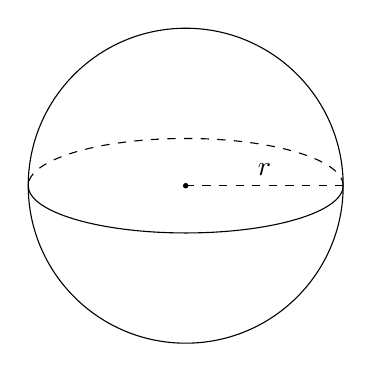
\begin{tikzpicture}
  \shade[ball color = white!40, opacity = 0] (0,0) circle (2cm);
  \draw (0,0) circle (2cm);
  \draw (-2,0) arc (180:360:2 and 0.6);
  \draw[dashed] (2,0) arc (0:180:2 and 0.6);
  \fill[fill=black] (0,0) circle (1pt);
  \draw[dashed] (0,0 ) -- node[above]{$r$} (2,0);
\end{tikzpicture}
\caption{\label{fig:kula}Kula}
\end{figure}

\begin{equation}
\label{eqn.kulaPole}
\mathrm{P}=4\pi r^2
\end{equation}

\begin{equation}
\label{eqn.kulaObjetosc}
\mathrm{V}=\frac{4}{3}\pi r^3
\end{equation} 

\newpage
\listoftables
\listoffigures
\end{document}